\section{Evaluation}%
\label{sec:evaluation}
\subsection{Graphs of Loss over Time}%
\label{sub:graphs_of_loss_over_time}
\begin{figure}[htpb]
    \centering
    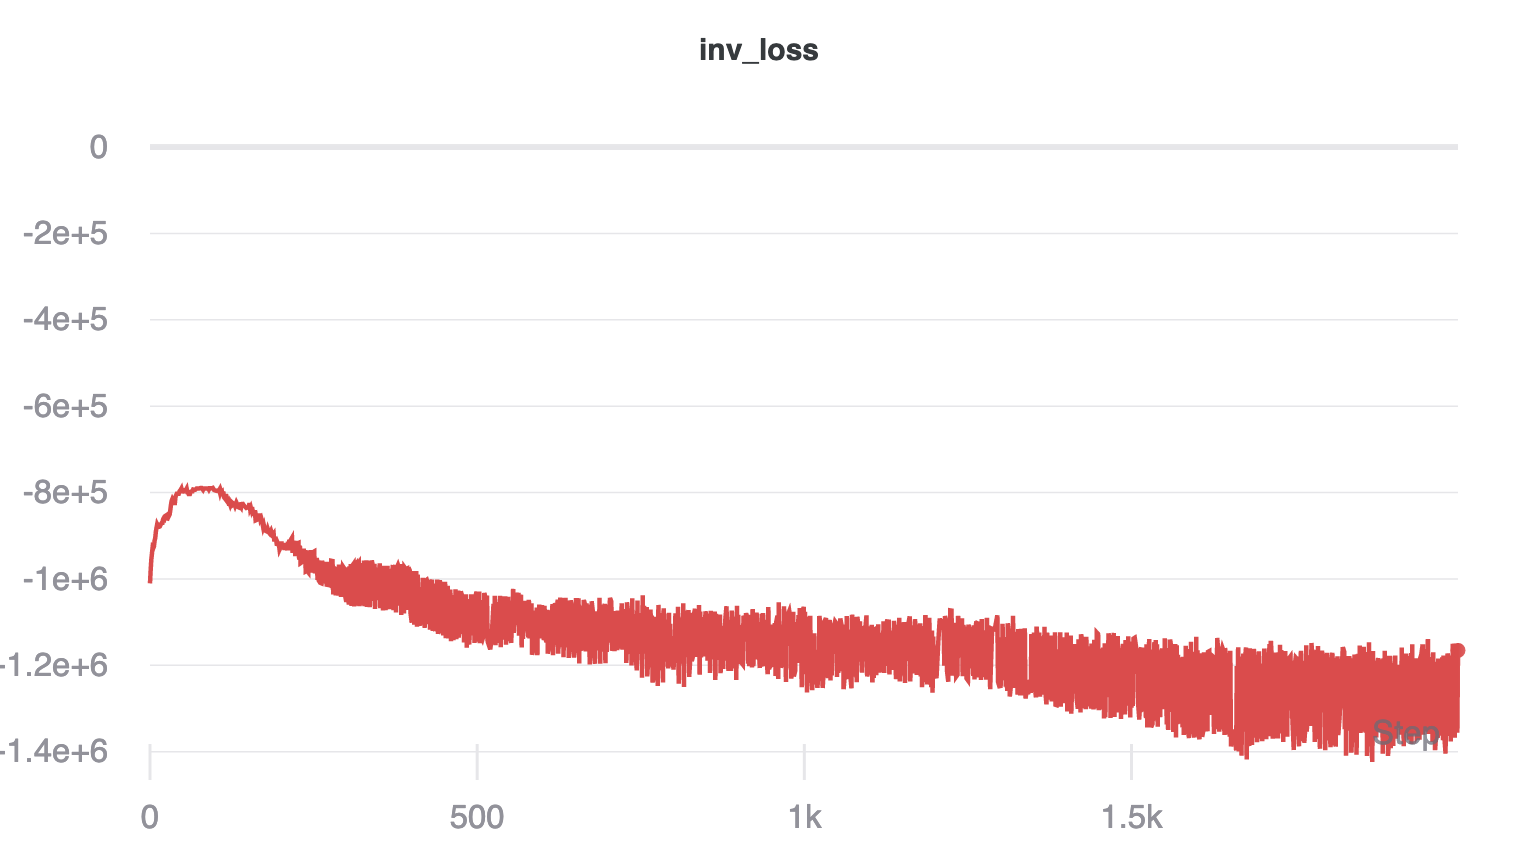
\includegraphics[width=0.8\linewidth]{images/invloss.png}
    \caption{Negative of Maximum Deviation vs Iterations}%
\end{figure}
\begin{figure}[htpb]
    \centering
    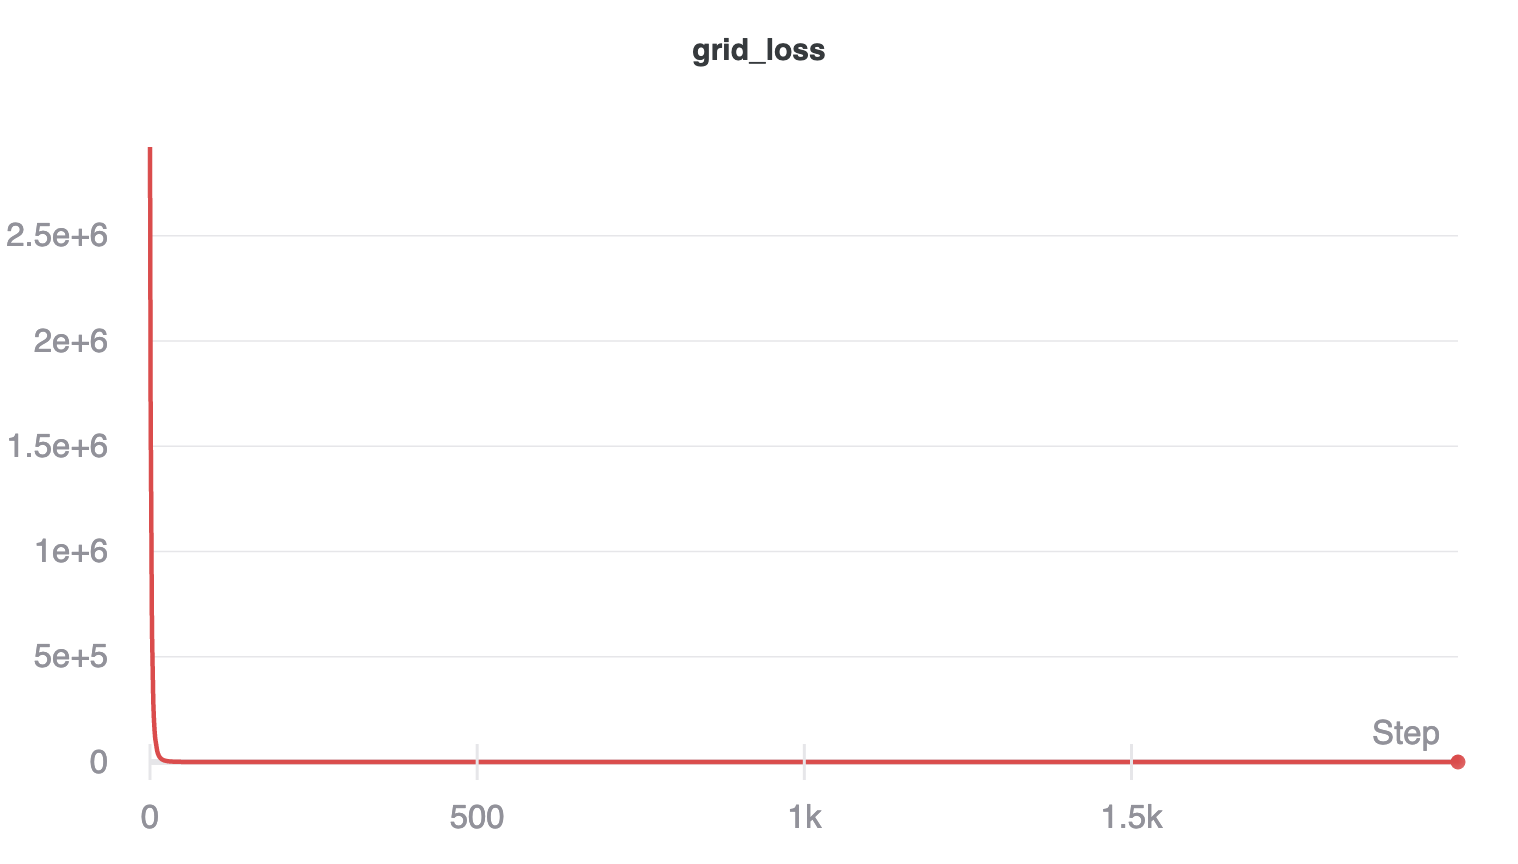
\includegraphics[width=0.8\linewidth]{images/gridloss.png}
    \caption{Superposition Loss vs Iterations}%
\end{figure}
\begin{figure}[htpb]
    \centering
    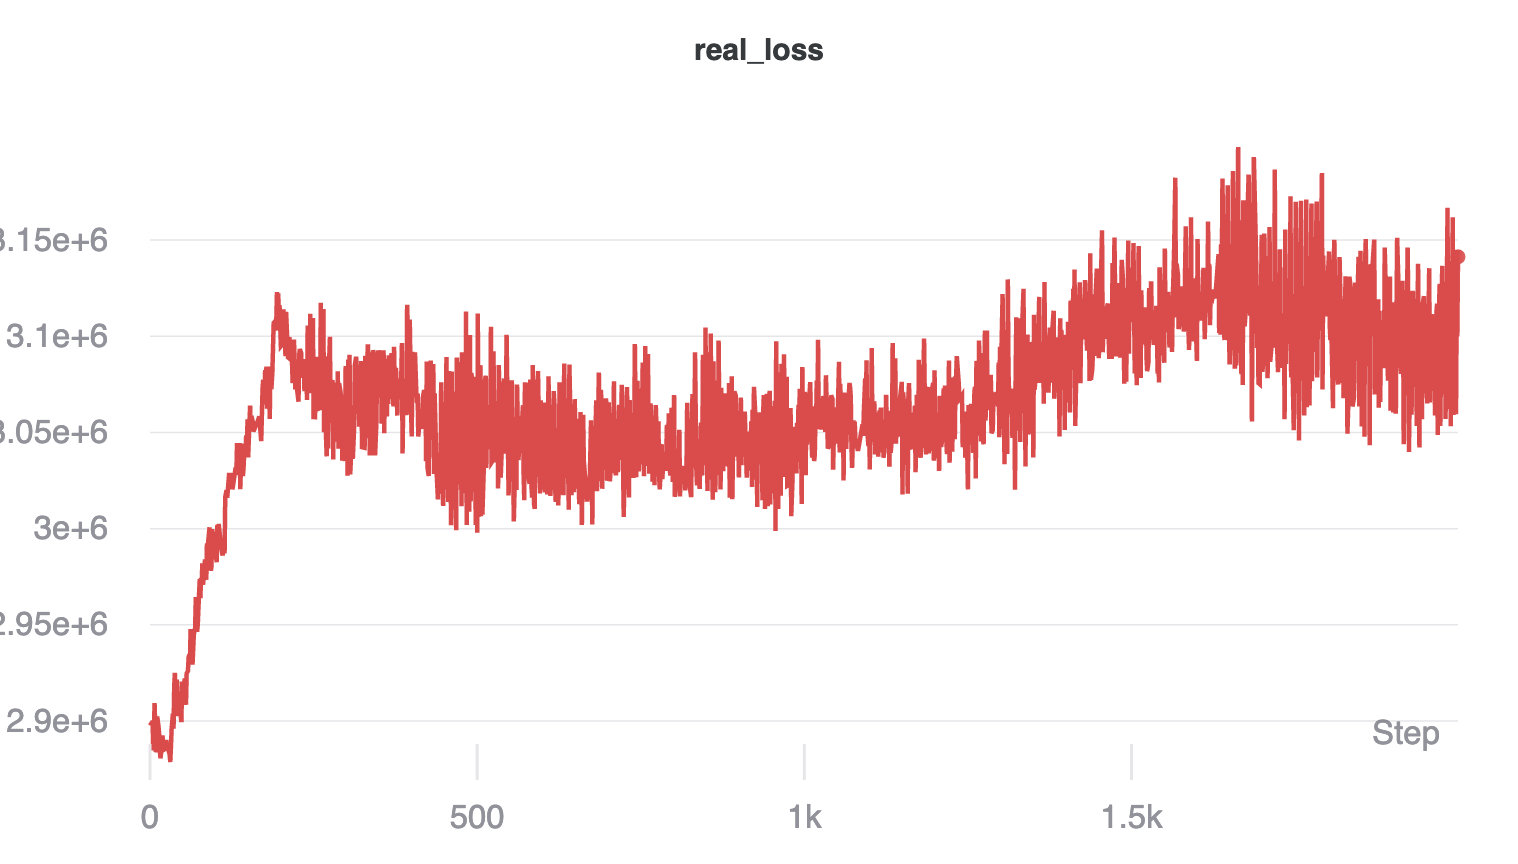
\includegraphics[width=0.8\linewidth]{images/real_loss.png}
    \caption{Discretized Grid Loss vs Iterations}%
\end{figure}

From the following images, we can see that Gradient Descent is in fact viable for Toroidal Grid Optimization \emph{in its continuous representation}, and that its success does not translate well over to the discretized version of the grid. This is reflected by the fact that the discretized loss after the optimization is worse off than it was in the beginning, during random initialization. This reflects a clear discrepancy between continuous and discrete optimization. The non-smoothness of 2 of the graphs can be traced to the non-discrete natures of both of those losses.

\subsection{Limitations}%
\label{sub:limitations}
A multi-objective loss function is difficult to optimize by nature. How much each component affects the overall loss function is to be determined arbitrarily, and these hyper-parameters\footnote{Parameters that cannot be learnt}, have to be tested arbitrarily. In this essay, only a single set of hyperparameters such as learning rate, proportion of negative maximum deviation and toroidal grid loss is used. This essay by no means provides a comprehensive evaluation of the possible optimization strategies, and therefore, may lack to optimize the function because of the wrong tuning of these hyperparameters and not a mistaken problem formulation.

The second possible reason is that I have not properly enforced the idea of discreteness within the optimization. There are a plentiful amount of methods to attempt this, including the Sinkhorn-Knopp algorithm for doubly stochastic matrices, and normal standard deviation. But through my trials, all of them work just about the same, which does not say a lot.

\subsection{Summary}%
\label{sub:summary}
Gradient descent is truly an amazing optimization algorithm. That is, if your loss function reflects the objective. But in the case of toroidal grid optimization, that does not seem to be the case. The stark difference between the continuous and the discrete nature of the problem of toroidal grid optimization makes gradient descent not a viable choice for this problem, according to the experiments laid out within this essay. But this does not hinder the effectiveness of Gradient Descent, but rather it highlights how it should be used properly. With a continuous objective.


